\documentclass[a4paper,14pt]{extarticle}
\usepackage{../../tex-shared/report-layout}

\renewcommand{\mylabnumber}{2}
\renewcommand{\mylabtitle}{Исследование методов принятия решений в условиях стохастической неопределенности}
\renewcommand{\mysubject}{Поддержка принятия решений в условиях неопределенности}
\renewcommand{\mylecturer}{Кротов К.В.}

\begin{document}
\begin{titlepage}
    
    \thispagestyle{empty}
    
    \begin{center}
        
        Министерство науки и Высшего образования Российской Федерации \\
        Севастопольский государственный университет \\
        Кафедра ИС
        
        \vfill

        Отчет \\
        по лабораторной работе №\mylabnumber \\
        \enquote{\mylabtitle} \\
        по дисциплине \\
        \enquote{\MakeTextUppercase{\mysubject}}

    \end{center}

    \vspace{1cm}

    \noindent\hspace{7.5cm} Выполнил студент группы ИС/б-17-2-о \\
    \null\hspace{7.5cm} Горбенко К. Н. \\
    \null\hspace{7.5cm} Проверил \\
    \null\hspace{7.5cm} \mylecturer

    \vfill

    \begin{center}
        Севастополь \\
        \the\year{}
    \end{center}

\end{titlepage}

\section{Цель работы}
Изучить и исследовать методы принятия решений при наличии информации о
стохастической связи между экспериментами и их исходами, между принимаемыми
решениями и их результатами.

\section{Задание на работу}
Для дерева принятия решений, представленного на \ref{fig:tree}, и
соответствующих этому дереву распределений вероятностей, выполнить определение
эффективных стратегий проведения эксперимента и принятия решений с
использованием метода анализа дерева решений в экстенсивной форме. Таблицы
распределений вероятностей, состав множеств экспериментов, исходов, решений и
состояний системы сформировать самостоятельно в соответствии с видом дерева.

\begin{figure}[H]
    \centering
    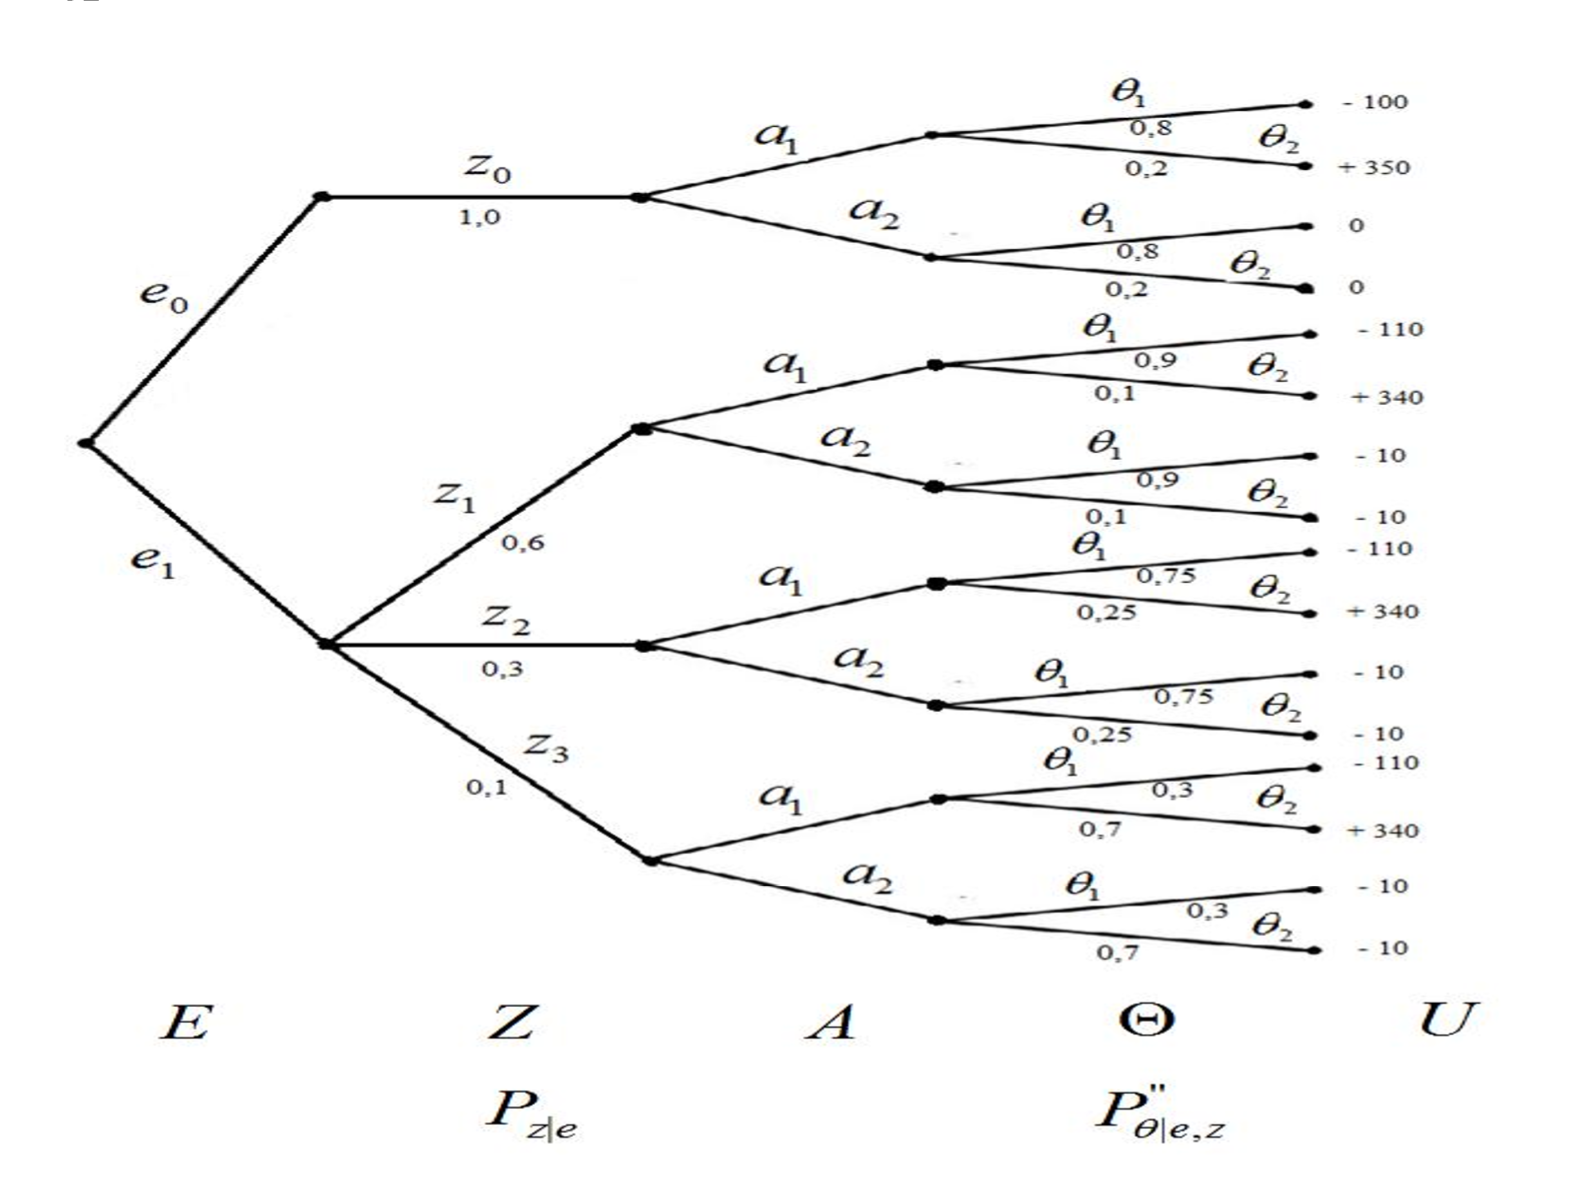
\includegraphics[width=.8\linewidth]{tree}
    \caption{Дерево принятия решений}
    \label{fig:tree}
\end{figure}
\pagebreak

\section{Ход работы}
Текст программы:

\begin{lstlisting}
const int P_TETA_COUNT = 1;
const int A_COUNT = 2;
const int TETA_COUNT = 2;
const int Z_COUNT = 4;
const int E_COUNT = 2;
void createMatrix(float** &matrix, int row, int col);
void printMatrix(float** matrix, int row, int col);
void readFile_Matrix(string name, int n, int numCollmus,float** matrix);
int main()
{float** P_TetaMatrix;float** P_Z_EMatrix;float** P_Teta_ZMatrix;float**** Umatrix;
char choice;string P_TetaFile="D:\\1.txt";string P_Z_EFile="D:\\2.txt";
string P_Teta_ZFile="D:\\3.txt";ifstream UFile("D:\\4.txt");
createMatrix(P_TetaMatrix, TETA_COUNT, P_TETA_COUNT);
createMatrix(P_Z_EMatrix, Z_COUNT, E_COUNT);
createMatrix(P_Teta_ZMatrix, TETA_COUNT, Z_COUNT);
	UMatrix = new float***[E_COUNT];
	for (int i = 0; i < E_COUNT-1; i++) {
		UMatrix[i] = new float**[Z_COUNT];
		for (int j = 0; j < Z_COUNT; j++){
			UMatrix[i][j] = new float*[A_COUNT];
			for (int l = 0; l < A_COUNT; l++)	{
				UMatrix[i][j][l] = new float[TETA_COUNT];	}	}	}
	readFile_Matrix(P_TetaFile, TETA_COUNT, P_TETA_COUNT,P_TetaMatrix);
	readFile_Matrix(P_Z_EFile, Z_COUNT, E_COUNT,P_Z_EMatrix);
	readFile_Matrix(P_Teta_ZFile, TETA_COUNT, Z_COUNT,P_Teta_ZMatrix);
	for (int i = 0; i < E_COUNT-1; i++)
	{
		for (int j = 0; j < Z_COUNT; j++)
		{
			for (int l = 0; l < A_COUNT; l++)
			{
				for (int k = 0; k < TETA_COUNT; k++)
				{
					UFile >> UMatrix[i][j][l][k];
				}	}}}
	cout << "P_Teta matrix" << endl;
	printMatrix(P_TetaMatrix, TETA_COUNT, P_TETA_COUNT);
	cout << "P_Z_E matrix" << endl;
	printMatrix(P_Z_EMatrix, Z_COUNT, E_COUNT);
	cout << "P_Teta_Z matrix" << endl;
		printMatrix(P_Teta_ZMatrix, TETA_COUNT, Z_COUNT);
	cout << "U matrix" << endl;
		for (int i = 0; i < E_COUNT - 1; i++)
		{
			for (int j = 0; j < Z_COUNT; j++)
			{
				for (int k = 0; k < A_COUNT; k++)
				{
					for (int l = 0; l < TETA_COUNT; l++)	{
						cout << UMatrix[i][j][k][l] << " "		}}}}
		cout << endl;
	//1
	float* U_EZA_massive = new float[Z_COUNT*A_COUNT];
	for (int i = 0; i < Z_COUNT*A_COUNT; i++)
	{	U_EZA_massive[i] = 0;}
	for (int h = 0; h < E_COUNT-1; h++)
	{	for (int i = 0, l = 0; i < Z_COUNT; i++)
		{	for (int j = 0; j < A_COUNT; j++)	{
				for (int k = 0; k < TETA_COUNT; k++)		{		
					U_EZA_massive[l] += UMatrix[h][i][j][k] * P_Teta_ZMatrix[k][i];
				}l++;	}}}	cout << "U(e,z,a): " << endl;
	for (int i = 0; i < Z_COUNT*A_COUNT; i++)	{
		cout << U_EZA_massive[i] << " ";}cout << endl;
	//2
	float* U_EZ_massive = new float[Z_COUNT];
	for (int i = 0; i < Z_COUNT; i++){
		U_EZ_massive[i] = 0;}
	float max;
	for (int i = 0, j=0; i < Z_COUNT; i++)	{
		max = U_EZA_massive[j];
		for (int l = 0; l < TETA_COUNT; l++)	{
			if (U_EZA_massive[l+j] > max)
			{			max = U_EZA_massive[l+j];
			}		}		U_EZ_massive[i] = max;
		j += A_COUNT;	}
	cout << "U(e,z): " << endl;
	for (int i = 0; i < Z_COUNT; i++)	{
		cout << U_EZ_massive[i] << " ";}
	cout << endl;
	//3
	float* U_E_massive = new float[E_COUNT];
	for (int i = 0; i < E_COUNT; i++)
	{	U_E_massive[i] = 0;}
	U_E_massive[0] = U_EZ_massive[0];
	for (int i = 1, l = 1 ; i < E_COUNT; i++)
	{	for (int k = 1; k < Z_COUNT; k++)
		{
			U_E_massive[i] += U_EZ_massive[k] * P_Z_EMatrix[k][i];
		}	}	cout << "U(e): " << endl;
	for (int i = 0; i < E_COUNT; i++)	{
		cout << U_E_massive[i] << " ";	}
	cout << endl;
	//4
	float best_solution = U_E_massive[0];
	for (int i = 1; i < E_COUNT; i++)	{
		if (U_E_massive[i] > best_solution)	{
			best_solution = U_E_massive[i];	}	}
	cout << "\n U* = " << best_solution<<endl;
	int a_number=0;
	int e_number=0;
	for (int i = 0; i < Z_COUNT*A_COUNT; i++){
		if (U_EZA_massive[i] == best_solution)
		{	a_number = i + 1;}
		if (U_E_massive[i] == best_solution)		{
			e_number = i;
		}	}	cout << "answer: e"<<e_number<<", a"<<a_number<< endl;
	cin.get();getchar();return 0;}
void createMatrix(float** &matrix, int row, int col)
{matrix = new float*[row];
	for (int i = 0; i < row; i++){
		matrix[i] = new float[col];}}
void printMatrix(float** matrix, int row, int col){
	for (int i = 0; i < row; i++){
		for (int j = 0; j < col; j++){
			cout << matrix[i][j] << " ";}
		cout << endl;}cin.get();}
void readFile_Matrix(string name, int n, int numCollums, float** matrix) {
	FILE *inp; int i,j;
		if ((inp = fopen(name.c_str(), "r")) == NULL){
		cout<< "Error by open" <<endl;
		return;}
	else
	for (i = 0; i<n; i++)		for (j = 0; j<numCollums; j++)
        fscanf(inp, "\%f", &matrix[i][j]);		fclose(inp);
}
\end{lstlisting}

\begin{figure}[H]
    \centering
    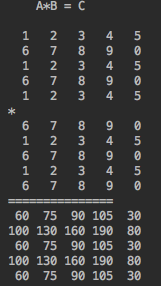
\includegraphics[width=.6\linewidth]{result}
    \caption{Результат работы программы}
    \label{fig:result}
\end{figure}

\section*{Выводы}
В ходе выполнения лабораторной работы исследовали методы принятия решений при
наличии информации о стохастической связи между экспериментами и их исходами,
между принимаемыми решениями и их результатами. По дереву принятия решений
заполнили таблицы вероятностей, написали программу, обрабатывающую таблицы и
определяющую эффективное решение.

\end{document}